%----------------------------------------------------------------------------------------
%	PACKAGES AND OTHER DOCUMENT CONFIGURATIONS
%----------------------------------------------------------------------------------------

\documentclass[18pt]{extarticle}

%%%%%%%%%%%%%%%%%%%%%%%%%%%%%%%%%%%%%%%%%
% Lachaise Assignment
% Structure Specification File
% Version 1.0 (26/6/2018)
%
% This template originates from:
% http://www.LaTeXTemplates.com
%
% Authors:
% Marion Lachaise & François Févotte
% Vel (vel@LaTeXTemplates.com)
%
% License:
% CC BY-NC-SA 3.0 (http://creativecommons.org/licenses/by-nc-sa/3.0/)
% 
%%%%%%%%%%%%%%%%%%%%%%%%%%%%%%%%%%%%%%%%%

%----------------------------------------------------------------------------------------
%	PACKAGES AND OTHER DOCUMENT CONFIGURATIONS
%----------------------------------------------------------------------------------------

\setlength{\parindent}{0em}
\setlength{\parskip}{.5em}

\usepackage{amsmath,amsfonts,stmaryrd,amssymb} % Math packages

\usepackage{enumerate} % Custom item numbers for enumerations

\usepackage[ruled]{algorithm2e} % Algorithms

\usepackage[framemethod=tikz]{mdframed} % Allows defining custom boxed/framed environments

\usepackage{dirtytalk}

\usepackage{listings} % File listings, with syntax highlighting
\lstset{
	basicstyle=\ttfamily, % Typeset listings in monospace font
}

\usepackage{hyperref}
\hypersetup{
    colorlinks=true,
    linkcolor=blue,
    filecolor=magenta,      
    urlcolor=cyan,
}


%----------------------------------------------------------------------------------------
%	DOCUMENT MARGINS
%----------------------------------------------------------------------------------------

\usepackage{geometry} % Required for adjusting page dimensions and margins

\geometry{
	paper=a4paper, % Paper size, change to letterpaper for US letter size
	top=2.5cm, % Top margin
	bottom=3cm, % Bottom margin
	left=2.5cm, % Left margin
	right=2.5cm, % Right margin
	headheight=14pt, % Header height
	footskip=1.5cm, % Space from the bottom margin to the baseline of the footer
	headsep=1.2cm, % Space from the top margin to the baseline of the header
	%showframe, % Uncomment to show how the type block is set on the page
}

%----------------------------------------------------------------------------------------
%	FONTS
%----------------------------------------------------------------------------------------

\usepackage[utf8]{inputenc} % Required for inputting international characters
\usepackage[T1]{fontenc} % Output font encoding for international characters

\usepackage{XCharter} % Use the XCharter fonts

%----------------------------------------------------------------------------------------
%	COMMAND LINE ENVIRONMENT
%----------------------------------------------------------------------------------------

% Usage:
% \begin{commandline}
%	\begin{verbatim}
%		$ ls
%		
%		Applications	Desktop	...
%	\end{verbatim}
% \end{commandline}

\mdfdefinestyle{commandline}{
	leftmargin=10pt,
	rightmargin=10pt,
	innerleftmargin=15pt,
	middlelinecolor=black!50!white,
	middlelinewidth=2pt,
	frametitlerule=false,
	backgroundcolor=black!5!white,
	frametitle={Command Line},
	frametitlefont={\normalfont\sffamily\color{white}\hspace{-1em}},
	frametitlebackgroundcolor=black!50!white,
	nobreak,
	singleextra={%
    }
}

% Define a custom environment for command-line snapshots
\newenvironment{commandline}{
	\medskip
	\begin{mdframed}[style=commandline]
}{
	\end{mdframed}
	\medskip
}

%----------------------------------------------------------------------------------------
%	FILE CONTENTS ENVIRONMENT
%----------------------------------------------------------------------------------------

% Usage:
% \begin{file}[optional filename, defaults to "File"]
%	File contents, for example, with a listings environment
% \end{file}

\mdfdefinestyle{file}{
	innertopmargin=1.6\baselineskip,
	innerbottommargin=0.8\baselineskip,
	topline=false, bottomline=false,
	leftline=false, rightline=false,
    leftmargin=0cm,rightmargin=0cm,
	singleextra={%
		\draw[fill=black!10!white](P)++(0,-1.2em)rectangle(P-|O);
		\node[anchor=north west]
		at(P-|O){\ttfamily\mdfilename};
		%
		\def\l{3em}
		\draw(O-|P)++(-\l,0)--++(\l,\l)--(P)--(P-|O)--(O)--cycle;
		\draw(O-|P)++(-\l,0)--++(0,\l)--++(\l,0);
	},
	firstextra={%
		\draw[fill=black!10!white](P)++(0,-1.2em)rectangle(P-|O);
		\node[anchor=north west]
		at(P-|O){\ttfamily\mdfilename};
		%
	},
    middleextra={%
    },
    secondextra={%
		\def\l{3em}
		\draw(O-|P)++(-\l,0)--++(\l,\l)--(P)--(P-|O)--(O)--cycle;
		\draw(O-|P)++(-\l,0)--++(0,\l)--++(\l,0);
    },
    nobreak,
}

% Define a custom environment for file contents
\newenvironment{file}[1][File]{ % Set the default filename to "File"
	\medskip
	\newcommand{\mdfilename}{#1}
	\begin{mdframed}[style=file]
}{
	\end{mdframed}
	\medskip
}

%----------------------------------------------------------------------------------------
%	NUMBERED QUESTIONS ENVIRONMENT
%----------------------------------------------------------------------------------------

% Usage:
% \begin{question}[optional title]
%	Question contents
% \end{question}

\mdfdefinestyle{question}{
	innertopmargin=1.2\baselineskip,
	innerbottommargin=0.8\baselineskip,
	roundcorner=5pt,
	singleextra={%
		\draw(P-|O)node[xshift=1em,anchor=west,fill=white,draw,rounded corners=5pt]{%
		Άσκηση \theQuestion\questionTitle};
	},
	firstextra={%
		\draw(P-|O)node[xshift=1em,anchor=west,fill=white,draw,rounded corners=5pt]{%
		Άσκηση \theQuestion\questionTitle};
	},
}

\newcounter{Question} % Stores the current question number that gets iterated with each new question

% Define a custom environment for numbered questions
\newenvironment{question}[1][\unskip]{
	\bigskip
	\stepcounter{Question}
	\newcommand{\questionTitle}{~#1}
	\begin{mdframed}[style=question]
}{
	\end{mdframed}
	\medskip
}

%----------------------------------------------------------------------------------------
%	WARNING TEXT ENVIRONMENT
%----------------------------------------------------------------------------------------

% Usage:
% \begin{warn}[optional title, defaults to "Warning:"]
%	Contents
% \end{warn}

\mdfdefinestyle{warning}{
	topline=false, bottomline=false,
	leftline=false, rightline=false,
	nobreak,
	singleextra={%
		\draw(P-|O)++(-0.5em,0)node(tmp1){};
		\draw(P-|O)++(0.5em,0)node(tmp2){};
		\fill[black,rotate around={45:(P-|O)}](tmp1)rectangle(tmp2);
		\node at(P-|O){\color{white}\scriptsize\bf !};
		\draw[very thick](P-|O)++(0,-1em)--(O);%--(O-|P);
	}
}

% Define a custom environment for warning text
\newenvironment{warn}[1][Warning:]{ % Set the default warning to "Warning:"
	\medskip
	\begin{mdframed}[style=warning]
		\noindent{\textbf{#1}}
}{
	\end{mdframed}
}

%----------------------------------------------------------------------------------------
%	INFORMATION ENVIRONMENT
%----------------------------------------------------------------------------------------

% Usage:
% \begin{info}[optional title, defaults to "Info:"]
% 	contents
% 	\end{info}

\mdfdefinestyle{info}{%
	topline=false, bottomline=false,
	leftline=false, rightline=false,
	nobreak,
	singleextra={%
		\fill[black](P-|O)circle[radius=0.4em];
		\node at(P-|O){\color{white}\scriptsize\bf i};
		\draw[very thick](P-|O)++(0,-0.8em)--(O);%--(O-|P);
	}
}

% Define a custom environment for information
\newenvironment{info}[1][Info:]{ % Set the default title to "Info:"
	\medskip
	\begin{mdframed}[style=info]
		\noindent{\textbf{#1}}
}{
	\end{mdframed}
}

\newcommand{\src}[1]{{\texttt{#1}}}

 % Include the file specifying the document structure and custom commands

%----------------------------------------------------------------------------------------
%	ASSIGNMENT INFORMATION
%----------------------------------------------------------------------------------------

\title{Χρόνο-προγραμματισμός Διεργασιών στο \src{xv6} Kernel \\Λειτουργικά Συστήματα (ECE ΓΚ702)} % Title of the assignment

\author{\footnotesize Χρήστος Φείδας\\ \footnotesize \src{fidas@upatras.gr} \and \footnotesize Ευάγγελος Λάμπρου\\ \footnotesize \src{e.lamprou@upnet.gr}} % Author name and email address

\date{University of Patras --- \the\year{}} % University, school and/or department name(s) and a date

%----------------------------------------------------------------------------------------
\bibliography{bibliography}

\begin{document}

\pagestyle{fancy}
%... then configure it.
\fancyhf{} % sets both header and footer to nothing
\renewcommand{\headrulewidth}{0pt}
\fancyhead{} % clear all header fields
\fancyfoot{} % clear all footer fields
\fancyfoot[L]{\footnotesize Χρήστος Φείδας, \footnotesize Ευάγγελος Λάμπρου}
\fancyfoot[R]{\thepage}

\maketitle

\tableofcontents

%----------------------------------------------------------------------------------------
%	INTRODUCTION
%----------------------------------------------------------------------------------------

\section{Εισαγωγή}

Ο χρονοπρογραμματισμός διεργασιών είναι μία από τις σημαντικότερες 
αρμοδιότητες ενός λειτουργικού συστήματος.
Στόχος είναι η κάθε διεργασία να \say{νομίζει} πως έχει ένα 
δικό της CPU στο οποίο εκτελούνται σειριακά οι εντολές της.
Αν αυτό ήταν αλήθεια βέβαια, θα χρειαζόμασταν $n$ επεξεργαστικές μονάδες 
για να εκτελέσουμε $n$ διεργασίες ταυτόχρονα στον υπολογιστή μας. 
Μέσω της πολύπλεξης διεργασιών γίνεται να φαίνεται πως τρέχουν ταυτόχρονα στον υπολογιστή μας
πολύ περισσότερες διεργασίες απ'ότι οι πυρήνες που κατέχει το σύστημά μας.

Στο xv6 η πολύπλεξη αυτή γίνεται με την CPU να εναλλάσεται από τη μία διεργασία
στην άλλη σε περιπτώσεις
\begin{enumerate*}
    \item Μηχανισμός sleep και wake % TODO cite
    \item CPU time interrupt σε περίπτωση που μία διεργασία εκτελείται για μεγάλο χρονικό διάστημα
\end{enumerate*}

\subsection{Context Switching}

\begin{figure}[H]
    \centering
    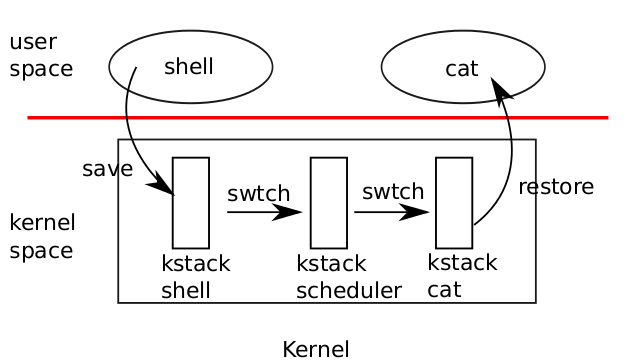
\includegraphics[width=0.4\textwidth]{assets/sched/switch.png}
    \caption{Context switch από μία διεργασία χρήστη (\src{shell}) 
    προς μία ρουτίνα πυρήνα (\src{scheduler}) και τελικά 
    σε μία άλλη διεργασία χρήστη (\src{cat}).}
\end{figure}

\section{Προετοιμασία}

Θα συνεχίσετε πάνω στον πηγαίο κώδικα της προηγούμενης εργασίας. 
Για αρχή, ενώ είστε μέσα στο φάκελο \src{xv6}, εκτελέστε τις παρακάτω \src{git} εντολές
ώστε να φτιάξετε ένα νέο branch πάνω στο οποίο θα κάνετε τις νέες αλλαγές. Αυτό 
θα το κάνει εύκολο να πάτε πίσω στο αρχικό branch σε περίπτωση λαθών.

\begin{commandline}
\begin{verbatim}
$ git chechout -b scheduling 
\end{verbatim}
\end{commandline}

\subsection{Προτεινόμενο Διάβασμα}

\begin{itemize}

    \item Διαβάστε από το βιβλίο του xv6 \cite{xv6Book} το κεφάλαιο 5 (\textit{Scheduling})
    \item Δείτε το επεξηγηματικό \href{https://www.youtube.com/watch?v=-O_JX5mMMHY}{βίντεο} για μία λεπτομερή παρουσίαση της διαδικασίας scheduling στο xv6.

\end{itemize}

\section{Ασκήσεις}

\begin{question}
    Πώς αναπαρίσταται μία διεργασία στο xv6 kernel;
    Εξηγήστε τη σημασία καθενός από τα members του struct 
    το οποίο αντιπροσωπεύει μία διεργασία στο σύστημα.

    \begin{info}[Σημείωση:]
        Κοιτάξτε στο αρχείο \src{kernel/proc.h}.
    \end{info}
\end{question}

\begin{question}
    Ποια είναι η συνάρτηση \src{scheduler}, ποια είναι η συνάρτηση \src{sched} και ποια είναι η διαφορά τους;
\end{question}

% \begin{question}
%     Υλοποιήστε την συνάρτηση \src{scheduler} ώστε να υποστηρίζει την πολιτική προγραμματισμού First Come, First Served (FCFS).
% \end{question}

\begin{question}
    Επεξεργαστείτε την συνάρτηση \src{scheduler} ώστε να υποστηρίζει την πολιτική προγραμματισμού Lottery Scheduling \cite{OSTEP-SchedLottery, LotteryScheduling1994}

    Το Lottery Scheduling θα λειτουργεί ως εξής:

    Μία διεργασία ξεκινά την εκτέλεσή της με ένα συγκεκριμένο αριθμό εισητηρίων (\src{tickets}), αυτό μπορεί να είναι ένας οποιοδήποτε αριθμός θέλετε.
    Ο scheduler κάνει μια κλήρωση για την κάθε διεργασία. Αν κάποια από αυτές \say{κερδίσει}, θα ξεκινήσει η εκτέλεσή της.
    Αυτή η διαδικασία θα επαναλαμβάνεται για κάθε κλήση στον scheduler.

    Ο αριθμός εισητηρίων μιας διεργασίας μπορεί να αλλάξει με τη χρήση της system call \src{settickets(int n)} που θα πρέπει να υλοποιήσετε.
    Όταν ο χρήστης εκτελεί αυτή τη system call, η τρέχουσα διεργασία θα αλλάζει αριθμό εισητηρίων με βάση το όρισμα. Η τρέχουσα διεργασία 
    που τρέχει στον πυρήνα βρίσκεται στην global μεταβλητή \src{proc} μέσα στο kernel.

    Τη διαδικασία της κλήρωσης μπορείτε να την υλοποιήσετε με διάφορους τρόπους.
    Μια απλή προσέγγιση είναι ο scheduler να υπολογίζει έναν τυχαίο αριθμό μεταξύ 0 και \src{total\_tickets}.
    Έπειτα, για την κάθε διεργασία να γίνεται έλεγχος αν ο αριθμός των εισητηρίων της είναι μεγαλύτερος από αυτό το νούμερο. Αν ναι, κερδίζει την κλήρωση.

    Θα χρειαστεί επίσης να προσθέσετε μία \href{https://wiki.osdev.org/Random_Number_Generator#Pseudorandom_number_generators}{γεννήτρια τυχαίων αριθμών} στο kernel.

    Για να καταλάβετε αν λειτουργεί σωστά ο scheduler σας μπορείτε να χρησιμοποιήσετε 
    το έτοιμο πρόγραμμα \src{sched-test}. Αυτό θα σας δώσει στατιστικά σχετικά με το χρόνο εκτέλεσης 
    της κάθε διεργασίας. Εξηγήστε γιατί η υλοποίησή σας είναι σωστή με βάση τα αποτελέσματα.
    Επεξεργαστείτε τον κώδικα στο αρχείο \src{user/sched-test.c} αλλάζωντας τον αριθμό των εισητηρίων 
    που δίνονται στην κάθε διεργασία. Εξηγήστε τα αποτελέσματα της εκτέλεσης.

    \begin{info}[Βοήθεια:]
        Τα σημεία του πηγαίου κώδικα που θα πρέπει να επεξεργαστείτε είναι τα εξής: 
        
        \begin{itemize}
            \item Συνάρτηση \src{scheduler} στο αρχείο \src{kernel/proc.c} ώστε να γίνεται η επιλογή της διεργασίας που θα εκτελεστεί σε κάθε κβάντο με βάση τον νικητή της κλήρωσης.
            \item Συνάρτηση \src{fork} στο αρχείο \src{kernel/proc.} μπορείτε να έχετε μία διεργασία να κληρονομεί τα εισητήρια από το γονέα της.
            \item Τα αρχεία \src{kernel/sysproc.c}, \src{kernel/syscall.c}, \src{include/sysproc.h}, \src{include/user.h}, \src{ulib/usys.S} 
                για την προσθήκη της απαραίτητης κλήσης συστήματος ώστε να ελέγχεται ο αριθμός εισητηρίων μιας διεργασίας από κώδικα χρήστη.
            \item Συμπληρώστε τον κατάλληλο κώδικα στο αρχείο \src{include/random.h} για την υλοποίηση της γεννήτριας τυχαίων αριθμών.
        \end{itemize}

        Φροντίστε να δώσετε στην διεργασία \src{init} (PID 1) ένα τουλάχιστον εισητήριο.
    \end{info}

\end{question}

\printbibliography

\end{document}
